\graphicspath{{content/introduction/figures/}}

\mychapter{Introduction}{chap:introduction}
\epigraph{\textit{``As a rule'', said Holmes, ``the more bizarre a thing is the
less mysterious it proves to be. It is your commonplace, featureless crimes which are
really puzzling, just as a commonplace face is the most difficult to
identify.''}}{---\textsc{Sherlock Holmes}} 

Programmers have always had to cope with change, it was ever-present in the
development of software and people did very little besides simply accepting it
as a given. Even though it was such a universal problem, the concept of handling
change in a consistent manner (i.e. \emph{refactoring}) was introduced only in
1990~\cite{first-ref-mention}, and the first tools to perform these changes
automatically were introduced only several years later.

Software engineers have had to manage, arguably, the most complex systems ever
built by humans for decades now. To this end they have adopted
\emph{refactorings} as a central tenant during the development process and have
grown to appreciate the user-friendly support of IDEs for these transformations,
especially for code written in the Java language. The automation of
refactorings, in turn, reveals an interesting concept: the separation of roles in
human-machine interaction. The programmer is responsible for the consistency of
the abstract, high-level concerns of the system, while the machine performs the
tedious and repetitive analyses and transformations necessary for performing
refactorings.

And now, with the effects of Moore's law beggining to fade the software
development community is forced to start refactoring for parallelism. The
difficulties raised by trying to make code execute \emph{correctly} in parallel
are non-trivial; add this to the fact that standard software systems are in of
themselves hard to manage, retrofitting old software to this new paradigm
becomes a very difficult problem.

\mysection{Contribution}{sec:contribution}

From the points raised above an obvious idea comes to mind: a tool that helps
the programmer transform sequential code into parallel code; thus freeing the
programmer from the burden of the tedious transformations done on legacy systems
whose performance no longer improves with new hardware. Such a tool exists in
the form of \emph{ReLooper} (presented bellow) and our contribution is extending
its functionality by offering a solution for fixing data-races using only static
analysis, see~\ref{th:static-analysis}.

\mysubsection{ReLooper}{th:ReLooper}
Briefly described, ReLooper~\cite{ReLooper} takes as input a user-selected loop
that performs computationally intensive operations on large data sets and
converts it using Java's \emph{ParalelArray}~\ref{th:parallel-array} data
structure which facilitates easy execution of parallel tasks on the array's
elements. This transformation can be performed only if the code that comprises
these tasks does not result in any data-races in the context of parallel
execution. It also does an analysis that determines such data-races.

\mysection{General overview of the algorithm}{sec:overview}

During an analysis of open source projects (see chapter~\ref{chap:analysis})
we've identified a common method for fixing data-races. Namely, make
data that was once shared between threads unique to each one; every thread getting its
own copy of the data. There are two ways of doing this:
\begin{enumerate} 
  \item [a)] by moving object allocation to the parallel context.
  \item [b)] encapsulate objects in Java's ThreadLocal~\ref{th:thread-local}, a wrapper
  class which ensures that the data enclosed is unique for each thread.
\end{enumerate}

We have named the transformations described above as \emph{data privatization},
which will be the term used hereafter. This thesis will focus mostly on the
second method, but with slight variations. Instead of \emph{ThreadLocal} we use
our own construct called \emph{ThreadPrivate} (see
chapter~\ref{ssec:threadprivate}) which behaves mostly like \emph{ThreadLocal},
but offers support for ensuring that the copy of the data that is referenced in
each of the threads is in the state in which it was before the execution of the
parallel operation.

We omitted the first one because it would have required reasoning mostly about
the program execution outside of the parallel context which usually spans much
larger parts of the program. And it would have had much stricter preconditions
because if we introduce \emph{ThreadLocal} in sequential parts of the program
the preserves the semantics of the original program; moving entire objects and
fields does not.

An abstract overview of the major computational tasks that our tool does in
order to perform the above mentioned transformation can be seen in
Figure~\ref{fig:generalalgo}.

\begin{figure}[h!]
	\begin{center}
		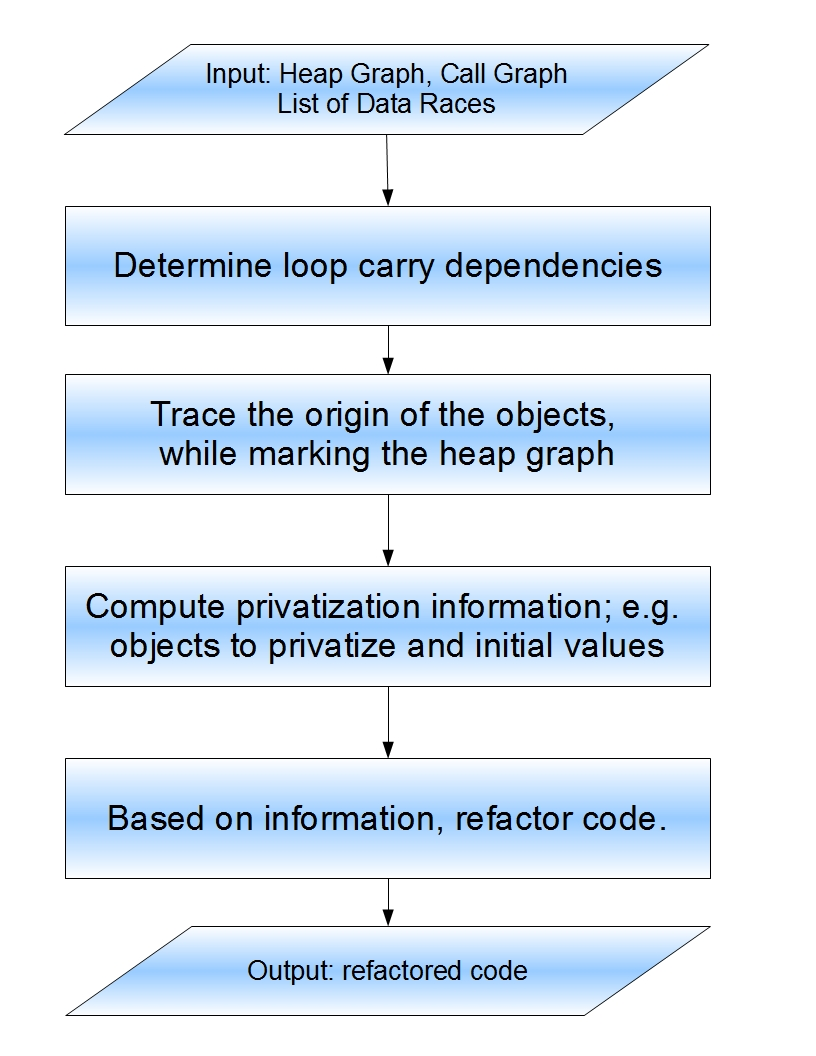
\includegraphics[width=8cm]{algo}
		\caption{Flow chart that depicts the major
		computational stages of the algorithm}
		\label{fig:generalalgo}
	\end{center}
\end{figure}

We take as input a list of data-races which are detected by an analysis that is
part of \emph{ReLooper}, determine which of these is a \slcd (see
definition~\ref{def:lcd}) because we cannot privatize data involved in this kind
of data-race without breaking the semantics of the program (see
chapter~\ref{chap:lcd}). Then we look to see where the data comes from in a
process we call access-trace; during which we mark the classes and fields that
have referenced this data before. This information helps us determine which
classes and fields are best to be refactored using \emph{ThreadPrivate} while
trying to minimize the amount of calls to its getters and setters in order to
avoid needless overhead.
Finally, we use a refactoring built on top of the \emph{eclipse IDE} to perform
the actual changes on the code.